\section{Interpretation Methods}
\label{sec:interpretation_methods}

There exists a variety of definitions in the vastly expanding research field of XAI, and the concept of \textit{interpretability} still has no formal commonly used technical meaning \cite{lipton2018mythos}. To build on the common ground of existing research, this work follows the terminology of Lipton et al. \cite{lipton2018mythos} and Arrieta et al. \cite{arrieta2020explainable}.

Broadly, interpretabiity focuses on \textit{how} and \textit{why} a machine learning model makes predictions.
Simply put, interpretability is focused on getting some notion of an explanation for the decisions made by a machine learning model.

%%%%%%%%%%%%%%%%%%%%%%%%%%%%%%%%%%%%%%%%%%%%%%
\subsection{Why is Interpretability Important?}
\label{subsec:importance_of_interpretability}

First, interpretability is helpful as it can help to build trust in a machine learning application. 
% Suppose a neural network predicts the risk for cancer from a mammogram, which is an image of breast tissue. A doctor would only use the algorithm if there is a way to validate that (1) tha algorithm is accurate (which can be measured in terms of the predictive accuracy), and (2) if the model is also using the correct indications in the data for predicting the risk of cancer. (1) is the standard approach for validating the performance of machine learning models, but in this example, one can clearly see why predictive accuracy might not be enough. For approaching (2), i.e. uncovering \textit{why} a model predicts a low / high risk of cancer, a variety of interpretation methods are proposed.  
% Ideally, an interpretation, or explanation method should indicate which pixels in the original image contribute to the prediction and also to what extent each pixel contributes. The extent to which each pixel contributes to a prediction is often called the \textit{importance} score of a feature. 

The advantage of post-hoc interpretations is that they do not interfere with the training process of the model, and thus do not change the model. As the name says, post-hoc means that the techniques can be easily applied to an already trained model without much further computational overhead. 

% https://thegradient.pub/interpretability-in-ml-a-broad-overview/ intro motvation
% https://towardsdatascience.com/why-how-interpretable-ml-7288c5aa55e4 also





High interpretability is desired as it can help to to uncover biases in the model. Suppose a machine learning model is to be deployed for the task of income prediction based on features such as age, race, gender, education and hours of work per week. The performance of the system would mainly be evaluated in terms oft the predictive accuracy and the fairness of the system. The former can be evaluated with metrics, such as accuracy on a held-out test set. For the latter, interpretability methods might be applied to observe which input features are used by the model to predict the income. 
% TODO note here that tha data from adult_income do actually not allow for these features to be more important than others. 
If the model uses sensitive features, such as sex and race as important features, it is systematically biased and thus unfair. 


%%%%%%%%%%%%%%%%%%%%%%%%%%%%%%%%%%%%%%%%%%%%%%
\subsection{Terminology}
\label{subsec:interpretation_methods_terminology}
The authors of \cite{arrieta2020explainable} make a distinction between the related but different concepts of \textit{interpretability} and \textit{explainibility}. Lipton \cite{lipton2018mythos} further breaks down interpretability into \textit{transparency} and \textit{post-hoc} interpretability. The notion of \textit{explainibility} from \cite{arrieta2020explainable} can be related to Liptons's \textit{transparency}, while Lipton's \textit{post-hoc} interpretability is essentially \textit{interpretability} as defined by Arrieta et al. \cite{arrieta2020explainable}.

\mypar{Post-hoc Interpretability} refers to the the extent to which cause and effect can be observed in a model, which can be translated to uncovering \textit{why} a model made prediction $y$ to an input $\mathbf{x}$, or how input and output ralate. Consider the example of image classification from \autoref{fig:bb}. Here, interpretability would mean that if a cat is present in the image (the cause), the model classifies it to the category 'cat' (the effect). Now imagine we find that the model takes the green meadow in the image as evidence to predict 'cat', and not the cat itself. This would imply a lack of interpretability, as the model learns to assign features to the concept 'cat' other than those related to 'cat' in the correct sense. This toy example emphasizes a common problem in image classification: \cite{xiao2020noise} observe the over-reliance of models on image background, rather than on objects in the foreground. % Note that interpretabe AI cannot verify if the learned relationships between features and outputs is truly causal (tha meadow in tha image can be correlated to the image category, e.g. when most images depictiong a cat shows cats on green meadows. This is a correlation of features but not necessarily a causilaty in tha sense of 'meadow --> cat'. ) https://www.pnas.org/content/pnas/116/44/22071.full.pdf causal inference
% Simply put, interpretability is focused on getting some notion of an explanation for the decisions made by a machine learning model.

\mypar{Explainibility or Transparency} on the other hand spans methods to uncover \textit{how} a model makes predictions, meaning to observe the inner workings of a model and thus to literally explain what is happening in terms of understanding of the mechanisms by which a model works. Thus, tansparency refers to the model's inherent properties that can be known before the training process and that are helpful to understand the model.

\par\smallskip
While both concepts seem to be important for the general objective of explainable artificial intelligence, this paper focuses on post-hoc interpretability.
There are essentially two ways to achieve interpretability: (1) to use inherently interpretable models or (2) to post-process a model in a fashion that allows to yield insights. The former is known as the development of \textit{surrogate} models and more generally described as \textit{model-agnostic} methods. Option (2) is known as \textit{model-transparent} methods. 

\mypar{Local and Global Methods.} A further categorization can be made based on the scope of interpretations: \textit{Local} methods aim at providing interpretations that are true for a single data points and its neighbors. 
\textit{Global} methods aim at gaining interpretations that are valid for most data points in a class \cite{kim2018interpretability, nguyen2017plug, yosinski2015understanding}. The interpretation methods discussed within this paper mostly fall into the class of local explanation methods \cite{ribeiro2016should, lundberg2017unified, bach2015pixel}. % TODO add all?

\mypar{Feature Attribution Methods and Sample Attribution Methods. } Interpretation methods aim at making complex and inherently uninterpretable black box models interpretable by creating human readable visualizations. 
A frequently used type of explanation methods are \textit{feature attributions} mapping each input feature to a numeric score. This score should quantify the importance of the feature relative to the model output. The resulting attribution map is then visualized as a heatmap projected onto the input sample. This allows humans to interpret which input attributes are the most helpful for making tha final prediction. Sample attribution methods on the other hand interpret the model performance in terms of the importance of training examples from the dataset. 

We propose the following formal definition for interpretation method:\newline

\textbf{Definition 1: Interpretation Method.}

\setlength{\leftskip}{0.39cm}

  \noindent We consider a neural network $N: \mathbb{R}^d \to \mathbb{R}^k$. For the an arbitrary classification task, $N$ classifies an input sample $\mathbf{x}\in \mathbb{R}$ in $k$ categories where the prediction $f_N(\mathbf{x})=y \in \{1, ..., K\}$ is given by $y = arg max_i f_N(\mathbf{x})_i$.

  Given the neural network $N$, it's input vector $\mathbf{x} \in \mathbb{R}^d$ and the the neural networks prediction for input $\mathbf{x}$, $f_N(\mathbf{x})=y$, an interpretation method $\mathcal{I}$ determines why label $y$ has been chosen by $N$ for input $\mathbf{x}$. 
  The interpretation is given by an output vector $\mathbf{h_k} \in \mathbb{R}^d$ for a class $k$ where each entry $h_i$ is mostly a numeric value describing the relevance for the $i$-th input feature $x_i$ of $\mathbf{x}$ for the final score $f_N(\mathbf{x})$.

\setlength{\leftskip}{0pt}
\par\smallskip\vspace{-0.1cm}

As $\mathbf{h}$ has the same dimensions as the input $\mathbf{x}$ it can be mapped to the input, overlaying $\mathbf{x}$ as a heatmap, where the color value represents the importance of feature $x_i$ towards the prediction $f_N(\mathbf{x})$.
An example is given in \autoref{fig:lrp_cat_lrp}. Higher values, implying a stronger relative importance for making the prediction $f_N(\mathbf{x})$, are depicted in dark red. 

% A model-transparent interpretation method, in the following named interpreter $\mathcal{I}$, generates a heatmap
%  $$h_c^\mathcal{I}(\boldsymbol{\omega}) = \mathcal{I}(\mathbf{x}, c; \boldsymbol{\omega})$$
%   for a neural network with parameters $\boldsymbol{\omega}$ and class $c$. The heatmap is a vector $h_c^\mathcal{I}(\boldsymbol{\omega}) \in \mathbb{R}^d$, where the $j$-th value $h_{c, j}^\mathcal{I}(\boldsymbol{\omega})$ represents the importance score of the $j-th$ input feature $x_j$ for the final score of class $c$.

While all explanation methods try to obtain importance measures for the network prediction, they differ with respect to how these measures are obtained. \cite{evaluating_explanations_security} propose two major categories for interpretation strategies, namely \textit{black-box}, in the following named \textit{model-agnostic} methods and \textit{white-box}, or \textit{} interpretation methods. 
While black-box interpretations assume no knowledge about the underlying model, white-box methods only work by using the model parameters. 

This terminology of discriminating between black-box and white-box methods may not be confused with the nature of the underlying models: Models still remain of black-box nature even though a white-box method may contribute to making the decision making process of such a model more insightful. % The opposite ofblack-box-nessistransparency,i.e., the search for a direct understanding of the mechanism by which a model works [5] 


The following section details the two categories and will give examples of the state-of-the-art interpretation methods within each group. 

% \noindent\textbf{Black-box Methods.} Black-box interpretations assume no knowledge about the model thus treating it as a black-box. The underlying model is approximated by learning it's behavior with an interpretable model, e.g. a linear model. As the model itself does not need to be known for using such a model-agnostic approach, thy can be used in scenarios where the model itself is not directly accessible. A black-box interpretation offers the big advantage to be applicable to any model.


% \noindent\textbf{White-box Methods.} On the other side are white-box interpretations, where the model is known with all its parameters. Thus, the explanations can be directly computed by using the model instead of relying on an approximation of $f_N$ as within the black-box models. As within these white-box models, tha model parameters can be used for calculating the interpretations, these methods are also named gradient or saliency map based methods. 

\subsection{Model-agnostic methods.}
\label{subsec:bb_methods}

% https://proceedings.neurips.cc//paper/2020/file/2c29d89cc56cdb191c60db2f0bae796b-Paper.pdf p. 4 
Model-agnostic interpretations assume no knowledge about the model thus treating it as a black box. The underlying model is approximated by learning it's behavior with an interpretable model, e.g. a linear model. The interpretable model is also dubbed the 'surrogate' model. The common approach for learning the surrogate is to approximate the relationship between the input samples and the corresponding prediction by tho model.
As the model itself does not need to be known, these approaches can be used in scenarios where the model itself is not directly accessible. Model-agnostic interpretations are fairly popular and are used in a wide range of applications, ranging from finance and law to medicine and chemistry \cite{elshawi2019interpretability, whitmore2016mapping}. 

A black-box interpretation offers the great advantage of being applicable to any model and offers simplicity because the interpretation is embedded in the model. However, this option of gaining interpretability might be costly for users that already have a high performing model. For this reason, growing need for methods exists that can be applied without retraining or modifying the underlying model.
We will briefly describe two common model-agnostic approaches. Refer to the original papers for details.

\mypar{Local Interpretable Model-agnostic Explanations (LIME).}\newline
LIME \cite{ribeiro2016should} perturbs the input and observes how the predictions of a black box model change. For the task of image classification, LIME creates a set of perturbed instances by dividing the input image into interpretable components, which are technically contiguous superpixels, and runs each perturbed instance through the model to get the probability for how much the change in each superpixel influences the whole model prediction. 

\autoref{fig:lime_cat} shows an example of LIME applied to the neural network model Inception-v3 \cite{szegedy2016rethinking}. Input image from the ImageNet dataset \cite{ILSVRC15}. The superpixel in dog instances place is highlighted in green, which correctly indicates that this superpixel has a high influence on the prediction of the images correct class ('bernese mountain dog'). LIME also correctly indicates that the superpixel in the cat's place does not indicate the correct class label.

\begin{figure}[ht]
  \centering
  \begin{subfigure}{0.32\linewidth}
    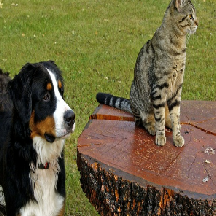
\includegraphics[width=\linewidth]{figures/lime_orig.png}
    \caption{Original}
    \label{fig:bird-a}
  \end{subfigure}
  \begin{subfigure}{0.32\linewidth}
    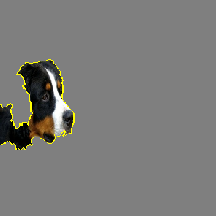
\includegraphics[width=\linewidth]{figures/lime_dog_mask.png}
    \caption{Mask.}
    \label{fig:bird-a}
  \end{subfigure}
  \begin{subfigure}{0.32\linewidth}
    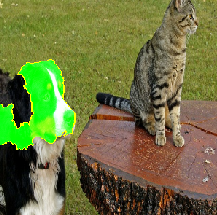
\includegraphics[width=\linewidth]{figures/lime_dog_map1.png}
    \caption{Saliency Map.}
    \label{fig:bird-a}
  \end{subfigure}
  \caption{Visualization of the output of the LIME interpreter applied to an image and image classification model.}\label{fig:lime_cat}
  \vspace{-0.3cm}
\end{figure}

% https://github.com/marcotcr/lime
% While the model may be very complex globally, it is easier to approximate it around the vicinity of a particular instance. While treating the model as a black box, we perturb the instance we want to explain and learn a sparse linear model around it, as an explanation. The figure below illustrates the intuition for this procedure. The model's decision function is represented by the blue/pink background, and is clearly nonlinear. The bright red cross is the instance being explained (let's call it X). We sample instances around X, and weight them according to their proximity to X (weight here is indicated by size). We then learn a linear model (dashed line) that approximates the model well in the vicinity of X, but not necessarily globally.


\mypar{SHapley Additive exPlanations (SHAP).} SHAP \cite{lundberg2017unified} builds on Shapley analysis, which is essentially about judging the importence of attibutes. The model is trained on a number of subsets of all available features, and the feature importance scores are calculated by evaluating the effects that the omissions of the specific features have on the model prediction. An example is shown in \autoref{fig:shap_dog}. Image regions highlighted in green are found to be important for predicting the correct label.

\begin{figure}[ht]
  \centering
  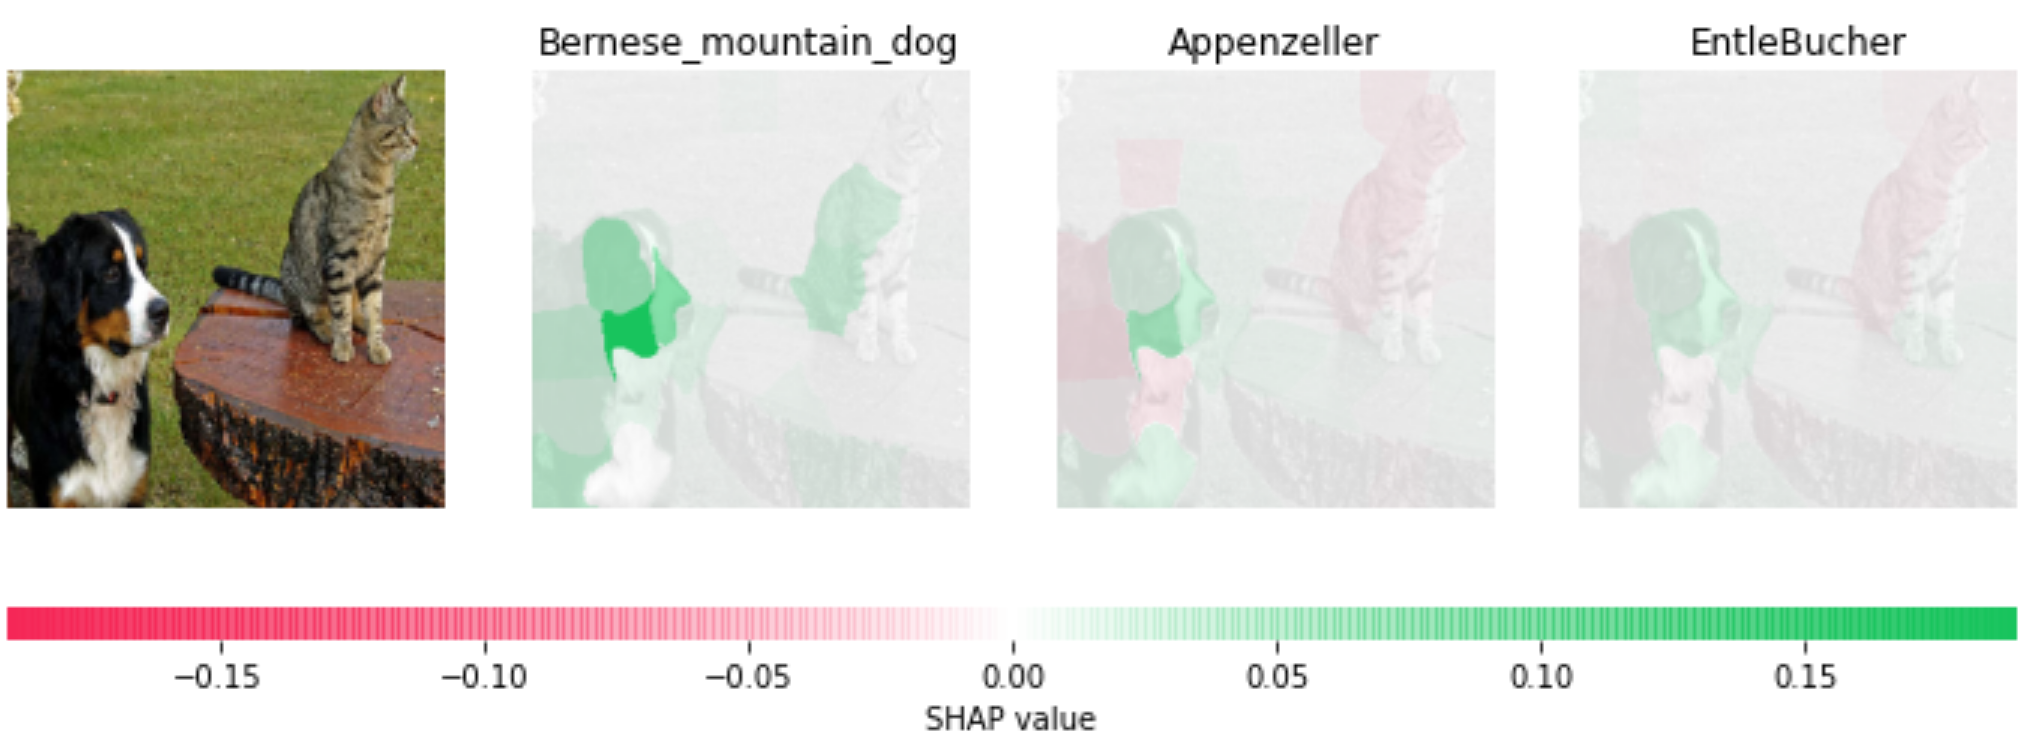
\includegraphics[width=\linewidth]{figures/cat_dog_shap.png}
  \caption{Visualization of the output of the SHAP interpreter applied to applied to an image and image classification model.}\label{fig:shap_dog}
  \vspace{-0.3cm}
\end{figure}


\subsection{Model-transparent methods.}
\label{subsec:wb_methods}

The other group of interpretations are model-transparent, or white-box methods, where the underlying model is known with all its parameters. Thus, the interpretation can be directly computed by using the model instead of relying on an approximation of $f_N$ as within the black-box methods. These methods typically rely on the relationship between an input sample, the underlying model's prediction and the associated activations of the models hidden layers. Methods within this group are for example propagation-based and gradient-based approaches. The former propagate back the model's prediction back through the model. The latter make use of the information provided by the gradients of the loss function, which contain sensitive information about the prediction and the features. Using the backpropagation method, features in the input can be highlighted based on the amount of gradient they receive. This shows their contribution to the final score. 
A few example methods within this group are listed below. 

\mypar{Layer-wise Relevance Propagation (LRP).} While many approaches in the group of model-transparent interpretations are designed only for image classification, or convolutional neural networks, this method \cite{bach2015pixel} is an exception. LRP propagates relevance values backwards through the network and decomposes the score of a predicted class backwards through the network. It relies on a Taylor series close to the prediction point rather than partial derivatives at the prediction point itself. An example for a feature map produced by LRP can be found in \autoref{fig:lrp_cat_lrp}.
%The output is a heatmap of relevance values, depicting for each feature how helpful or harmful the feature is for predicting the target class. 

\mypar{DeepLIFT} \cite{shrikumar2017learning} is an improved version of LRP, where a reference point in the input feature space is defined. Relevance scores are propagated proportionally to the changes of neuronal activations from the reference. % https://arxiv.org/pdf/1710.10547.pdf

\mypar{SmoothGrad (SG)} \cite{smilkov2017smoothgrad} avarages over interpretations of noisy copies of an input sample thus reducing noise by visually diffusing the interpretation. The noise is drawn from i.i.d. from a normal distribution. 

Methods developed for convolutional neural networks are for instace GradCAM \cite{selvaraju2017grad} or SimleGrad TODOcite. 
% \mypar{Gradient-weighted Class Activation Mapping (Grad-CAM)}
% Grad-CAM \cite{selvaraju2017grad} uses the gradients of any target concept, flowing into the final convolutional layer to produce a coarse localization map, highlighting the important regions in the image for predicting the concept.

% \mypar{SimpleGrad (SimpleG)}

% Please see the original publications for more detailed information. 